\documentclass[11pt, english]{article}
        \usepackage{geometry}
                \geometry{
                        a4paper,total={210mm,297mm},
                        tmargin=40.8mm,
                        bmargin=40.8mm,
                        lmargin=32.6mm,
                        rmargin=32.6mm,
                }

        \usepackage{titlesec}
                \titleformat{\section}
                        {\normalfont\fontsize{18}{16}\bfseries}{\thesection}{0.5em}{}
                \titleformat{\subsection}
                        {\normalfont\fontsize{14}{16}\bfseries}{\thesubsection}{1em}{}
                \titleformat{\subsubsection}
                        {\normalfont\fontsize{11}{16}\bfseries}{\thesubsubsection}{1em}{}

        \usepackage{longtable}
        \usepackage{multirow}

        \usepackage[labelfont=bf,textfont=bf,font=small,skip=8pt]{caption}

        \setlength{\parindent}{0pt}
        \renewcommand{\baselinestretch}{1.25}
        \usepackage{setspace}

        \usepackage{amsmath}
        \usepackage{amssymb}

	\usepackage{graphicx}

\begin{document}

\pagenumbering{gobble}

        \title{\textsc{AG215 Business Finance\\ Coursework Summary}}
        \author{\textsc{Lewis Britton}}
        \date{\textsc{Academic Year 2018/2019}}
        \maketitle

\newpage

\pagenumbering{roman}

        \renewcommand{\contentsname}{Table of Contents}

        \tableofcontents

\newpage

\pagenumbering{arabic}

\section{Capital Budgets}

	\subsection{Project A}

	\begin{center}
                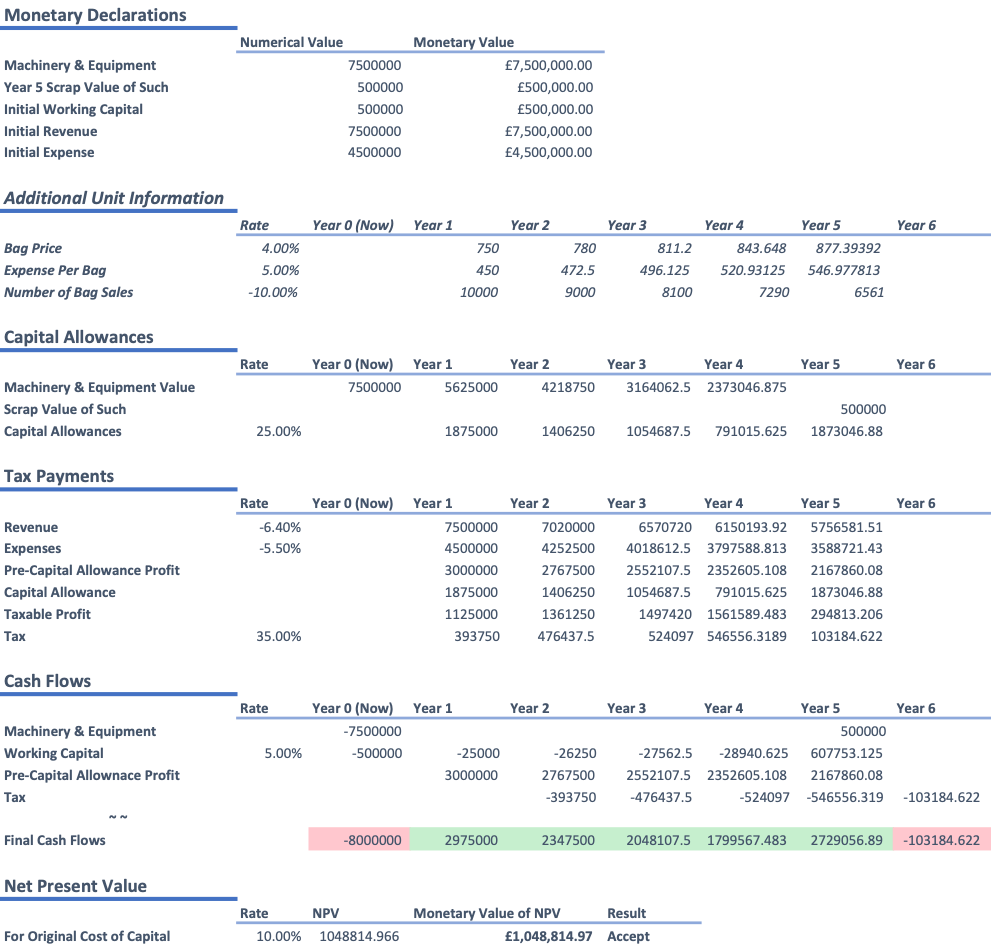
\includegraphics[height=14cm,width=14cm]{AG215-IMG/alpha.png}
        \end{center}

	\subsection{Project B}
                                                       
        \begin{center}                                 
                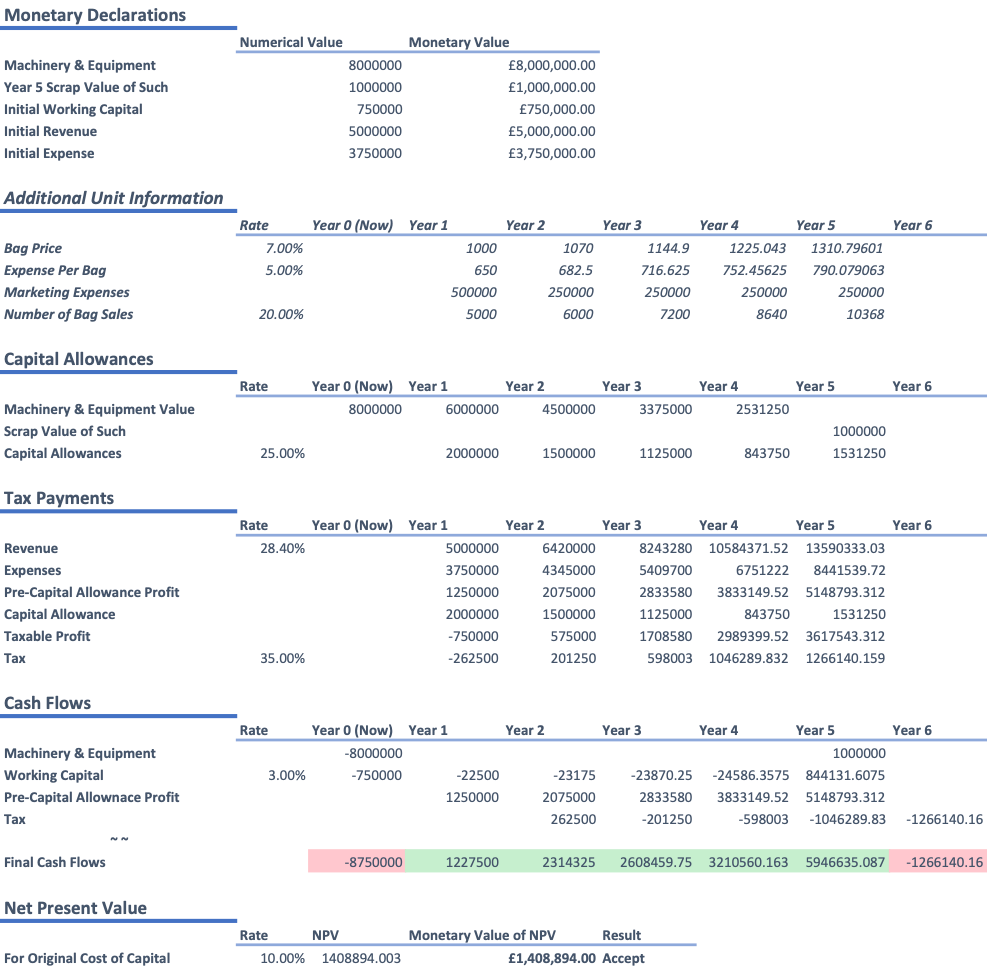
\includegraphics[height=14cm,width=14cm]{AG215-IMG/beta.png}
        \end{center}

	\subsection{Project A Analysis}

	The \textit{Monetary Declaration} section is self-explanatory as it simply contains given data from the brief in addition to Initial Revenue being calculated by multiplying the initial Bag Price by the initial Number of Bag Sales. And, Initial Expense being calculated by multiplying initial Expense Per Bag by the initial Number of Bag Sales. Hence, respectively:

	$$\mathrm{BP_{y1}*NoBS_{y1}}$$ $$\mathrm{EPB_{y1}*NoBS_{y1}}$$

	The \textit{Additional Unit Information} section shows the next year's Bag Price by multiplying the current one's by the given rate of 4\%. As follows:

	$$\mathrm{BP_{yx+1}=(BP_{yx}*(1+0.04))}$$

	Next, the calculating of the Expense Per Bag in the same manner at 5\% folows:

	$$\mathrm{EPB_{yx+1}=(EPB_{yx}*(1+0.05))}$$

	Finally, the Number of Bag Sales in the same manner again is calculated to observe the decrease in sales due to the negative rate, at 10\%. Hence: 

	$$\mathrm{NoBS_{yx+1}=(NoBS_{yx}*(1+(-0.10)))}$$

	The \textit{Capital Allowances} section shows first, calculating the Capital Allowance on Year $x$'s Machinery \& Equipment Value by multiplying this value by the rate, as follows:

	$$\mathrm{CA_{yx+1}=(MEV_{yx}*0.25)}$$

	Second, by subtracting this number from Year $x$'s Machinery \& Equipment Value to find Year ($x$ + 1)'s Machinery \& Equipment Value. This follows: 

	$$\mathrm{MEV_{yx+1}=(MEV_{y4}-SVoS_{y5})}$$

	Repeating until Year 4, resulting in Year 5's Capital Allowances being equal to Year 4's Machinery \& Equipment Value minus its Scrap Value in Year 5. That is:

	$$\mathrm{CA_{y5}=(MEV_{y4}-SVoS_{y5})}$$

	The \textit{Tax Payments} section refers to first, finding the Revenue and Expenses by multiplying the Number of Bag Sales values by the Bag Price and Expense Per Bag vaues, respectively for Years 2-5:

	$$\mathrm{R=(BP*NoBS)}$$ $$\mathit{E=EPB*NoBS}$$

	With Year 1's values being carried from earlier. Both R \& E decrease due to decreasing sales and increasing expenses therefore, have negative rates as shown. Next, Pre-Capital Allowance Profit is calculated by subtracting the Expenses from the Revenue for Years 1-5, as follows:

	$$\mathrm{PCAB=(R-E)}$$

	After the Capital Allowances have been carried, the Taxable Profit is calculated by subtracting the Capital Allowances form the Pre-Capital Allowances Profit as this tax does not apply to Capital Allowance, as follows:

	$$\mathrm{TP=(PCAB-CA)}$$

	Therefore, Tax is calculated by multiplying the Tax Rate by the Taxable Profit, as follows:

	$$\mathrm{T+(TP*(0.35))}$$

	Finally, the \textit{Cash Flows} section shows that by carrying the Taxes, carrying the Working Capital Rate and amending outflows to be negative, the Working Capital is be calculated by multiplying its Rate by the sum of all previous years’ Working Capital, as follows:

	$$\mathrm{WC=(SUM(WC_{y0}:WC_{yx})*(0.05))}$$

	All eligible flows are treated with regards to (*(-1)) for an outflow adjustment. The respective sums for flows of Machinery \& Equipment, Working Capital, Pre-Capital Allowance Profit and Tax lead to the Final Cash Flows which are increasing meaning overall profit increase, displayed as follows:

	$$\mathrm{FCF=(ME+WC+PCAP+T)}$$

	Hence, final Net Present Value (NPV) is as follows, relative to the first Cost of Capital rate:

	$$\mathrm{NPV=(0.10(SUM(FCF_{y1-6}))+(FCF_{y0}))}$$ $$\mathrm{NPV=0.10(2975000+2347500+204107.5+1799567.483+2729056.887}$$ $$\mathrm{-103184.6222)-8000000=1048814.97}$$

	This equates to \pounds1,048,814.97 which is greater than zero and therefore profitable. A \textit{Result} cell has been added based on an IF function, to reflect this.

	\subsection{Project B Analysis}

	All calculations in Project B are executed in the same manner as Project A’s, relative to Project B’s data with a few minor changes. The first being the Initial Expenses in Year 1, adjusted by the addition of 500000 for marketing expenses and 250000 added to each subsequent year’s Expenses, also for marketing, that is:

	$$\mathrm{E_{y2-5}=(EPB*NoBS)+ME_{y2-5}}$$

	$$\mathrm{ME=\textrm{Marketing Expenses}=2.5*10^5}$$

	The second note is, the Number of Bag Sales Rate is positive this time at 20\%; (1+0.20) and therefore results in increasing Revenues and Expenses, as rates of change for the Bag Price and Expense Per Bag are also positive. Despite the increased Expenses, this gives higher Pre-Capital Allowance Profit than Project A. Next, the Capital Allowance Rate changes to 3\% which simply alters the before seen formula to calculate the Working Capital, to multiply by 0.03. Giving smaller out flows here even with the higher initial Working Capital of -750000 being used as the multiplier rather than -500000 like before. Tax Rate remains the same and due to the higher Pre-Capital Allowance Profit, Taxable Profit is higher. All of these factors put together however, amount to far greater Final Cash Flows for Project B. Meaning there is proportionately enough marginal Revenue to make up for some higher Expenses. After the NPV calculation of: 

	$$\mathrm{NPV=(0.10,1227400+2314325+2608459.75+3210560.163+5946635.087-}$$ $$\mathrm{1266140.159)-8750000)=1408894.000}$$

	Therefore, an NPV of \pounds1,408,894.00 is given. This again, is greater than zero and thus, profitable.

	\subsection{Comparison, Conclusions \& Assumptions}

	In conclusion, this NPV is greater than Project A’s. As they are both above the breakeven point (NPV = 0), or Internal Rate of Return, both therefore are profitable. However, with no immediate complications or alterations, Project B offers a greater Net Present Value by \pounds360,079.04 and so, is more profitable. This most potently due to the, before described, positive increase in Number of Bag Sales per year, the higher increase rate of 7\%, rather than 4\%, in Bag Price and, the lowered Working Capital Rate. As these are multipliers, they can have a vital effect. Even though the overall Expenses are increasing in Project B, rather than decreasing, as in A and, Year 0 and Year 6 outflows were greater, the marginal increased Revenue is proportionately enough to bring Project B out on top. Making the Final Cash Flows for Project B not only higher than Project A’s but also, increasing by a greater amount. Thus, making Project B the most desirable project to proceed with.\\

	As for assumptions made regarding Project A, some existing required adaptation with a \pounds1,500,000 expense and therefore must be included as it is incremental to the project. Next, The Head Office charge for rental of the production grounds of \pounds500,000 is a Corporate Overhead and should therefore not be included. Initial Investments are taken as given. There were no apparent Sunk Costs, Opportunity Costs or Incidental Effects on the project. Working Capital is taken as given, the project suffers no Abandonment Costs. Taxes are paid at a constant rate of 35\% and, Tax Depreciation should be included to account for the Scrap Value of the machinery.\\

	Assumptions made in Project B include: a Sunk Cost of \pounds1,500,000 due to the money spent ``to date'' and therefore is not incremental to the project and is not included. Again, Initial Investments are taken as given. There were no apparent Opportunity Costs, Incidental Effects or Corporate Overheads. Working Capital is taken as given, the project suffers no Abandonment Costs. Taxes are paid at a constant rate of 35\% and, Tax Depreciation should be included to account for the Scrap Value of the machinery. Finally, for both projects, some ``Rates'' in the Spreadsheets are rates of change and some are simply applicable rates however, were both collected under the same column for form purposes.

\newpage

\section{Data Tables}

	\subsection{Project A}

	\begin{center}
        	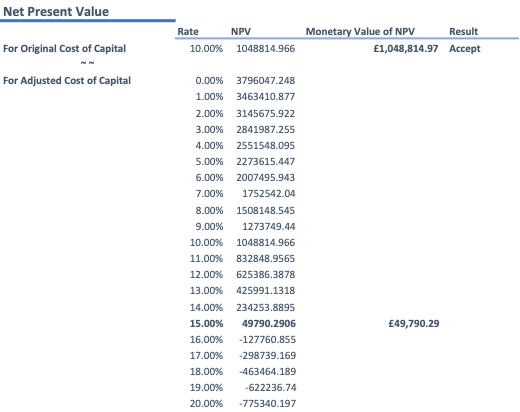
\includegraphics[height=8cm,width=10cm]{AG215-IMG/gamma.png}
        \end{center}

	\subsection{Project B}

	\begin{center}
               	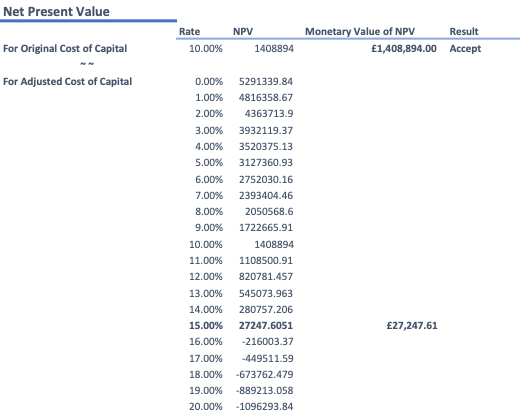
\includegraphics[height=8cm,width=10cm]{AG215-IMG/delta.png}
        \end{center}

	\subsection{Analysis}

	Using Data Tables, it can be seen in Project A, increasing the Cost of Capital rate to 15\% gives an NPV of £49,790.29. A 15\% Rate gives Project B an NPV of \pounds27,247.61. As we know, risk in Capital Budgeting can involve fluctuations and uncertainties in the market, tax, costs of manufacturing etc. and of course time. Examples include: accounting errors leading to unaccounted expenses and thus, higher Expenses; market demand of new features to the project hence, increasing the Expense increase rate; general forecasting being inaccurate leading to reduced Sales etc.; machinery/other unexpected failures leading to replacement/repair costs i.e. higher Expenses; possible macro-financial problems causing Abandonment mid-project; unpredicted Tax alterations, etc. These play a part in the uncertainty of projects and thus, determining an appropriate Cost of Capital rate. Therefore, these results show that even though Project B is more profitable, it is more sensitive to change as seen by the higher deviance in Project B’s results when the Cost of Capital rate is raised. Therefore, bringing the overall NPV down faster. Making Project B riskier and far more unreliable. Therefore, based on this analysis, this would change any immediate recommendations of Project B until further contemplation as Project A can be considered `safer'.

\newpage

\section{Sensitivity Analysis}	

	\subsection{Project A}

	\begin{center}
                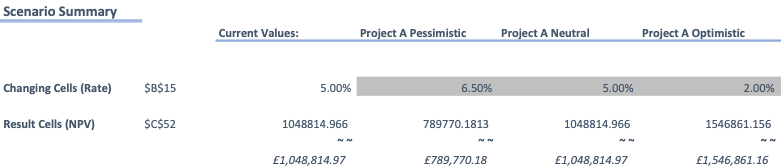
\includegraphics[height=2.5cm,width=12cm]{AG215-IMG/epsilon.png}
        \end{center}

	\subsection{Project B (I)}

	\begin{center}
                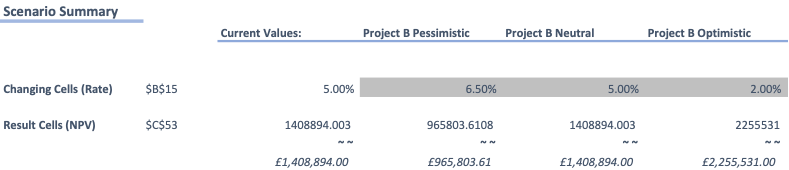
\includegraphics[height=2.5cm,width=12cm]{AG215-IMG/zeta.png}
        \end{center} 

	\subsection{Project B (II)}

        \begin{center}
                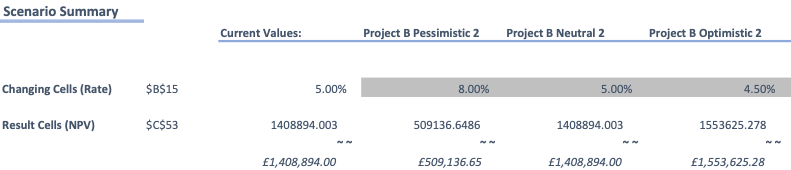
\includegraphics[height=2.5cm,width=12cm]{AG215-IMG/eta.png} 
        \end{center}

	\subsection{Analysis}

	First, Project A varies by roughly \pounds200,000 negatively when altered to 6.5\% and positively by roughly £500,000 when altered to 2\%. In terms of Project B, there is a decrease of roughly \pounds450,000 but an increase of around \pounds800,000, respectively. This again shows Project B is far more sensitive to the risk factors and uncertainty associated with the project as seen by the proportionately larger reaction to change. If it was realistic to reduce the Expense Per Bag rate to 2\% it would be a clear recommendation of Project B however, that is not reality and its most likely that the company, will over spend and increase the rate of growth in their Expense Per Bag. Therefore, Project A is safer in the worst possible event, making more of a profit when the rate is increased.\\

	Project B’s secondary suggested rates have simply put even more of a constraint on the best expected rate (4.5\%) to an increase in NPV of roughly \pounds150,000 but a decrease of almost \pounds1,000,000 when adjusted for the worst outcome of 8\%. This is more negatively impacting than both of the other projections and thus, solidifies the fact that Project B is far too unreliable. Project A appears to be the safest option in this scenario as even though its worst expected NPV lies below the, primary, worst expected NPV for B, it also lies above the, secondary, worst expected NPV for B. And, it contains a best possible NPV of \pounds1,546,861.16 which is very close to the, secondary, best expected NPV for B, \pounds1,553,625.28. Meaning, better results for A in a negative outcome and reasonably equal results in a positive outcome. Thus, A is more reliable.

\newpage

\section{Solver}

	\subsection{Project A}

	\begin{center}
		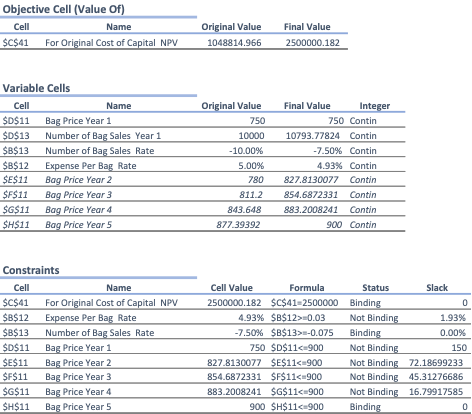
\includegraphics[height=8cm,width=10cm]{AG215-IMG/theta.png}
        \end{center}

	\subsection{Project B}

	\begin{center}
                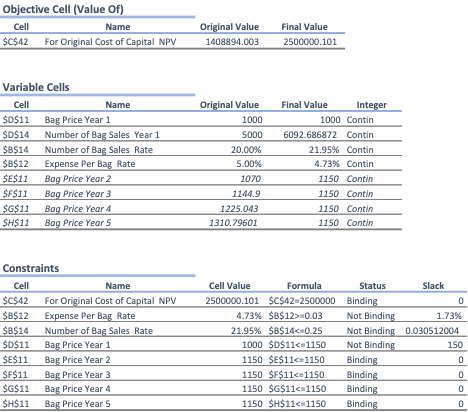
\includegraphics[height=8cm,width=10cm]{AG215-IMG/iota.png}
        \end{center}	

	\subsection{Analysis}

	As can be seen, it is possible to achieve the desired \pounds2.5m NPV, for both projects within an acceptable tolerance. By exhausting Solver, as it insisted on leaving Year 1 Bag Prices unchanged, it’s shown that to achieve the desired NPV in Project A, the Years 2-5 Bag Prices must be increased (remaining below \pounds900 as required), having reasonable slack. Number of Bag Sales Rate for growth increases by 1/4 with no slack, therefore pushing this to its allowable limit. Expense Per Bag Rate can also be decreased to a desirable value. And, Initial Bag Sales are increased by \~{}790, as desired. As for Project B, the same answer applies. Bag Prices for Years 2-5 must be increased and, stressed to the maximum possible value, i.e. no slack, making this risky. No. Bag Sales Rate for growth also increases but only by \~{}1/10 this time making this less desirable. Expense Per Bag Rate can also be decreased but, only by slightly more than Project A’s and with the other factors in Project A’s favour, this is essentially negligible.\\

	Therefore, the slack on Project B, and minor increases, are less meaningful as they relate to less controllable/predictable factors and less considerable increases where desired.

\end{document}
